%%%%%%%%%%%%%%%%%%%%%%%%%%%%%%%%%%%%%%%%%
%
% CIS530 final report - Michael Woods and Stuart Wagner
%
% Arsclassica Article
% LaTeX Template
% Version 1.1 (10/6/14)
%%%%%%%%%%%%%%%%%%%%%%%%%%%%%%%%%%%%%%%%%

%-------------------------------------------------------------------------------
%	PACKAGES AND OTHER DOCUMENT CONFIGURATIONS
%-------------------------------------------------------------------------------

\documentclass[
10pt, % Main document font size
a4paper, % Paper type, use 'letterpaper' for US Letter paper
oneside, % One page layout (no page indentation)
%twoside, % Two page layout (page indentation for binding and different headers)
headinclude,footinclude, % Extra spacing for the header and footer
BCOR5mm, % Binding correction
]{scrartcl}

%%%%%%%%%%%%%%%%%%%%%%%%%%%%%%%%%%%%%%%%%
% Arsclassica Article
% Structure Specification File
%
% This file has been downloaded from:
% http://www.LaTeXTemplates.com
%
% Original author:
% Lorenzo Pantieri (http://www.lorenzopantieri.net) with extensive modifications by:
% Vel (vel@latextemplates.com)
%
% License:
% CC BY-NC-SA 3.0 (http://creativecommons.org/licenses/by-nc-sa/3.0/)
%
%%%%%%%%%%%%%%%%%%%%%%%%%%%%%%%%%%%%%%%%%

%----------------------------------------------------------------------------------------
%	REQUIRED PACKAGES
%----------------------------------------------------------------------------------------

\usepackage[
nochapters, % Turn off chapters since this is an article        
beramono, % Use the Bera Mono font for monospaced text (\texttt)
eulermath,% Use the Euler font for mathematics
pdfspacing, % Makes use of pdftex’ letter spacing capabilities via the microtype package
dottedtoc % Dotted lines leading to the page numbers in the table of contents
]{classicthesis} % The layout is based on the Classic Thesis style

\usepackage{arsclassica} % Modifies the Classic Thesis package

\usepackage[T1]{fontenc} % Use 8-bit encoding that has 256 glyphs

\usepackage[utf8]{inputenc} % Required for including letters with accents

\usepackage{graphicx} % Required for including images
\graphicspath{{Figures/}} % Set the default folder for images

\usepackage{enumitem} % Required for manipulating the whitespace between and within lists

\usepackage{lipsum} % Used for inserting dummy 'Lorem ipsum' text into the template

\usepackage{subfig} % Required for creating figures with multiple parts (subfigures)

\usepackage{amsmath,amssymb,amsthm} % For including math equations, theorems, symbols, etc

\usepackage{varioref} % More descriptive referencing

%----------------------------------------------------------------------------------------
%	THEOREM STYLES
%---------------------------------------------------------------------------------------

\theoremstyle{definition} % Define theorem styles here based on the definition style (used for definitions and examples)
\newtheorem{definition}{Definition}

\theoremstyle{plain} % Define theorem styles here based on the plain style (used for theorems, lemmas, propositions)
\newtheorem{theorem}{Theorem}

\theoremstyle{remark} % Define theorem styles here based on the remark style (used for remarks and notes)

%----------------------------------------------------------------------------------------
%	HYPERLINKS
%---------------------------------------------------------------------------------------

\hypersetup{
%draft, % Uncomment to remove all links (useful for printing in black and white)
colorlinks=true, breaklinks=true, bookmarks=true,bookmarksnumbered,
urlcolor=webbrown, linkcolor=RoyalBlue, citecolor=webgreen, % Link colors
pdftitle={}, % PDF title
pdfauthor={\textcopyright}, % PDF Author
pdfsubject={}, % PDF Subject
pdfkeywords={}, % PDF Keywords
pdfcreator={pdfLaTeX}, % PDF Creator
pdfproducer={LaTeX with hyperref and ClassicThesis} % PDF producer
} 

\hyphenation{Fortran hy-phen-ation}

%-------------------------------------------------------------------------------
% TITLE AND AUTHOR(S)
%-------------------------------------------------------------------------------

\title{\normalfont\spacedallcaps{CIS530 Final Report}}

\author{\spacedlowsmallcaps{Stuart Wagner \& Michael Woods}}

\date{}

\begin{document}

%-------------------------------------------------------------------------------
% HEADERS
%-------------------------------------------------------------------------------

\renewcommand{\sectionmark}[1]{\markright{\spacedlowsmallcaps{#1}}} % The header for all pages (oneside) or for even pages (twoside)
%\renewcommand{\subsectionmark}[1]{\markright{\thesubsection~#1}} % Uncomment when using the twoside option - this modifies the header on odd pages
\lehead{\mbox{\llap{\small\thepage\kern1em\color{halfgray} \vline}\color{halfgray}\hspace{0.5em}\rightmark\hfil}} % The header style

\pagestyle{scrheadings} % Enable the headers specified in this block

%-------------------------------------------------------------------------------
% TABLE OF CONTENTS & LISTS OF FIGURES AND TABLES
%-------------------------------------------------------------------------------

\maketitle % Print the title/author/date block

\setcounter{tocdepth}{2} % Set the depth of the table of contents to show sections and subsections only

\tableofcontents % Print the table of contents

%-------------------------------------------------------------------------------
% INTRODUCTION
%-------------------------------------------------------------------------------

\section{Introduction}

Text classification on the basis of high or low information density has until
recently
\footnote{Nenkova \& Yang ``Detecting Information-Dense Texts in Multiple News Domains'' 2014 
\url{http://www.aaai.org/ocs/index.php/AAAI/AAAI14/paper/view/8430/8622}} 
been ignored. Building off the past research, we
seek to improve accuracy on classifying sentences with high information density.

Information density has several applications. Text summarization has relied
partially on the use of KL divergence--the measurement of a difference between
one distribution and another. However, this measure fails to account of
information density. Information dense sentences generally better summarize
information, as they more concisely describe information and ideas. Combined
with a summarizer, density classification could provide a more powerful and
precise text summarization.

Nenkova and Yang used a number of features in developing their model. We used
many similar features, however as students new to NLP, we instead thought that
using a variety of learners could provide better results. We therefore
approached the problem as a machine learning problem that leveraged NLP as
feature inputs. Could we learn which features were more important? Could we
leverage a variety of models, using ensemble learning, to improve accuracy? The
answer to those questions, generally speaking, is yes.

\newpage
 
%-------------------------------------------------------------------------------
% METHODS
%-------------------------------------------------------------------------------

\section{Methods and Resources}

We decided to frame the problem of classifying a given article as either 
information dense or sparse as primarilty a machine learning problem. As with
most problems that can be addressed with the methodologies of machine learning,
having some knowledge of the domain--in this case text classification--can 
provide useful insights when selecting and extract features from raw data. With 
the approaches we learned in CIS530 regarding the analysis of a text and
its structural componnts, along with our own intuitions and experimental 
insights, we outline the various features, tooling, and resources we employed 
for the project below.

\subsection{Data Resources}

% === MRC Psycholinguistic Database ===
\paragraph{\textbf{MRC Psycholinguistic Database}}
\hfill \newline \noindent \url{http://websites.psychology.uwa.edu.au/school/MRCDatabase/uwa_mrc.htm}
\hfill \newline \noindent The MRC Psycholinguistic Database is a machine readable
dictionary containing a number of linguistic and psycholinguistic
attributes and annotation for each word \footnote{\url{http://www.psych.rl.ac.uk/}}. 
Specifically, we primarily made use of the 4,923 lexicon included in the MRC 
distribution.

% === Linguistic Inquiry and Word Count (LIWC) ===
\paragraph{\textbf{Linguistic Inquiry and Word Count (LIWC)}}
\hfill \newline \noindent \url{http://www.liwc.net}
\hfill \newline \noindent The Linguistic Inquiry and Word Count (LIWC) is a text
analysis software program designed to calculate the degree to ``which people use 
different categories of words across a wide array of texts, including emails, 
speeches, poems, or transcribed daily speech''
\footnote{\url{http://www.liwc.net/}}.

\subsection{Tools and Software Packages}

% === Stanford CoreNLP ===
\paragraph{\textbf{Stanford CoreNLP}}
\hfill \newline \noindent \url{http://nlp.stanford.edu/software/corenlp.shtml}
\hfill \newline \noindent A suite of text processing tools capable of part-of-speech (POS) tagging, named
entity recognition (NER), tokenization, lemmatization, sentiment analysis, as
well as dependency and syntactic parse extraction.

% === scikit-learn ===
\paragraph{\textbf{scikit-learn}}
\hfill \newline \noindent \url{scikit-learn http://scikit-learn.org/}
\hfill \newline \noindent A popular Python machine learning framework with
implementations for a large selection of popular classifiers.

% === NumPy ===
\paragraph{\textbf{NumPy}}
\hfill \newline \noindent \url{http://www.numpy.org}
\hfill \newline \noindent A scientific computing package for Python providing 
native n-dimensional array datatype, as well as various linear algebra, 
statistical, and general mathematical functions suitable for ``''number crunching''.

% === NLTK ===
\paragraph{\textbf{NLTK}}
\hfill \newline \noindent \url{http://www.nltk.org/} 
\hfill \newline \noindent A popular Python library for working with natural 
language that includes a number of convenient text processing tools and built 
in corpora for multiple languages.

%------------------------------------------------

\subsection{Features}

Building off the work of Nenkova and Yang, we leveraged a number of similar 
features in our approach to the problem of textual information density
classification.

% === CoreNLP word count--binary bag-of-words ===
\paragraph{\textbf{CoreNLP word count--binary bag-of-words}} 
\hfill \newline \noindent \textit{9799 dimensions}. All unique tokens occurring
between \texttt{<word></word>} tags in the generated XML obtained from running all
training and test files through the CoreNLP tool were collected into a list and
converted to lowercase. Any tokens consisting of stop words, as defined by
NLTK's English stop word list or punctuation characters were removed. The list
was then sorted alphabetically in ascending order and each word was assigned an
index. To construct the feature vector for a given lead, the text of the lead
was processed in a manner similar to that of the XML output and a vector the
size of the bag-of-words model was initialized with zeros. If the lead contained
the $i$-th word in the bag-of-words model, the $i$-th position in the feature vector
was set to $1$.

% === CoreNLP sentence information ===
\paragraph{\textbf{CoreNLP sentence information}} 
\hfill \newline \noindent \textit{7 dimensions}. To construct the feature
vector, each processed lead had a number of pieces of information extracted from
it directly or from the XML file generated from it using CoreNLP. These
quantities define the features indicated below along with our prediction on it’s
impact on information density ($+$/$-$):
\begin{itemize}
	\item The number of sentences per lead. ($-$)
	\item The number of non-unique tokens per lead. ($-$)
	\item The number of named entities recognized in the lead. ($+$)
	\item The number of nouns in the lead (tokens tagged as \texttt{NN}, \texttt{NNS}, \texttt{NNP}, or \texttt{NNPS}) ($+$)
	\item The number of words with over six letters. ($+$)
	\item The number of quotation marks appearing in the lead. ($+$)
	\item The aggregate absolute sentiment score of the lead. Each sentence was assigned a numeric score according to the following rubric: ``very negative'': $2$, ``negative'': $1$, ``neutral'': $0$, ``positive'': $1$, and ``very positive'': $2$. The scores were then summed and the absolute value was taken. ($-$)
\end{itemize}

% === CoreNLP production rule count--binary bag-of-words ===
\paragraph{\textbf{CoreNLP production rule count--binary bag-of-words}} 
\hfill \newline \noindent \textit{5654 dimensions}. The syntactic parse
generated by CoreNLP for each sentence from a given lead is extracted from the
corresponding \texttt{<parse></parse>} tag in the corresponding XML file. A
parse tree is constructed in the same manner as described in Homework 3, where
only non- terminal nodes are considered. To construct the master list of
production rules, the outlined process is repeated for every lead file in the
training and test set and every unique production rule is collected into a list.
Each rule is then assigned an index, $0$ to $N-1$, where N is the number of
unique production rules. Then, to construct a feature vector for a given lead, a
$1 x N$ vector of zeros is created and every production rule occurring in the
sentences of the lead is extracted. For every rule in the master list, if the
$i$-th rule occurs in the rules extracted from the lead, the $i$-th index in the
feature vector is set to $1$. The belief was that perhaps certain production rules
may be related with information density.

% === LIWC ===
\paragraph{\textbf{LIWC}}
\hfill \newline \noindent \textit{78 dimensions}. Our hypothesis was that words
indicating sentiment and emotions might indicate sentences that were less
information dense. We thought these might be positively correlated with
information density: present tense, numbers, impersonal pronouns, and causation.
We also believed multiple attributes may be negatively correlated, including:
1st person usage, auxillary verbs and past tense, quantifiers, and positive and
negative emotion.

% === LIWC ===
\paragraph{\textbf{MRC dictionary--binary bag-of-words}}
\hfill \newline \noindent \textit{4923 dimensions}. 
The MRC Psycholinguistic database word dictionary consisting of $4,923$ words was
used to construct a binary bag-of-words model in a similar manner to the CoreNLP
binary bag-of-words model. We also attempted counts normalized by length of
lead, however there did not appear to be a significant difference in accuracy.
The text of each lead was tokenized, converted to lowercase and stripped of stop
words. The benefit of using this approach is that the dictionary is independent
of the task and training data (Nenkova and Yang).

%------------------------------------------------

\subsection{Models}
Regarding the actual task of classification, we constructed several 
classification models using the features described above. The model 
configurations are as follows:

\begin{itemize}
	\item Logistic regression with a L2 penalty and class weights $1$: $0.58$ and
	$-1$: $0.42$ set to reflect the true distribution of labels in the test set.

	\item Linear SVM regression with L2 loss and penalty functions and class 
	weights $1$: $0.58$ and $-1$: $0.42$ set to reflect the true distribution of 
	labels in the test set.

	\item Bernoulli naive bayes with default parameters.

	\item Ensemble method with the three classifiers described above. Each 
	classifier makes a prediction for a given observation and a majority vote
	is taken to determine the final predicted label.

\end{itemize}

%-------------------------------------------------------------------------------
%	RESULTS AND DISCUSSION
%-------------------------------------------------------------------------------

\section{Results and Discussion}

%------------------------------------------------

\subsection{Subsection}

\lipsum[11] % Dummy text

\subsubsection{Subsubsection}

\lipsum[12] % Dummy text

\begin{description}
\item[Word] Definition
\item[Concept] Explanation
\item[Idea] Text
\end{description}

\lipsum[12] % Dummy text

\begin{itemize}[noitemsep] % [noitemsep] removes whitespace between the items for a compact look
\item First item in a list
\item Second item in a list
\item Third item in a list
\end{itemize}

\subsubsection{Table}

\lipsum[13] % Dummy text

\begin{table}[hbt]
\caption{Table of Grades}
\centering
\begin{tabular}{llr}
\toprule
\multicolumn{2}{c}{Name} \\
\cmidrule(r){1-2}
First name & Last Name & Grade \\
\midrule
John & Doe & $7.5$ \\
Richard & Miles & $2$ \\
\bottomrule
\end{tabular}
\label{tab:label}
\end{table}

Reference to Table~\vref{tab:label}. % The \vref command specifies the location of the reference

%------------------------------------------------

\subsection{Figure Composed of Subfigures}

Reference the figure composed of multiple subfigures as Figure~\vref{fig:esempio}. Reference one of the subfigures as Figure~\vref{fig:ipsum}. % The \vref command specifies the location of the reference

\lipsum[15-18] % Dummy text

\begin{figure}[tb]
\centering
\subfloat[A city market.]{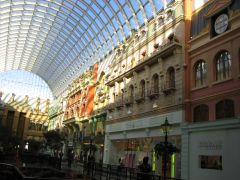
\includegraphics[width=.45\columnwidth]{Lorem}} \quad
\subfloat[Forest landscape.]{
\includegraphics[width=.45\columnwidth]{Ipsum}\label{fig:ipsum}} \\
\subfloat[Mountain landscape.]{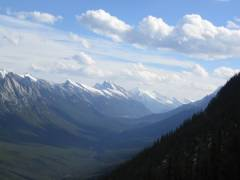
\includegraphics[width=.45\columnwidth]{Dolor}} \quad
\subfloat[A tile decoration.]{
\includegraphics[width=.45\columnwidth]{Sit}}
\caption[A number of pictures.]{A number of pictures with no common theme.} % The text in the square bracket is the caption for the list of figures while the text in the curly brackets is the figure caption
\label{fig:esempio}
\end{figure}

%-------------------------------------------------------------------------------

\end{document}